
\chapter{Objekte und Schnitttests}\label{ch:obj_schnitt}

Bis jetzt ist der "`Raytracer"' in der Lage Strahlen gemäß eines gewünschten Kameramodells in die Szene zu schicken. Der nächste Schritt besteht nun darin, die Szene mit Objekten zu bevölkern. Anschließend muss überprüft werden, ob ein ausgesandter Strahl eines der Objekte trifft. Im Falle, dass mehrere Objekte hintereinander liegen und es somit zu mehreren Schnitten kommt, wird immer der Schnittpunkt gesucht, der dem Betrachter am nächsten ist. Abb.~\ref{fig:schnitt_objekte} zeigt einen solchen Fall. Die Durchdringung der Objekte, wird durch Verwendung des zum Betrachter nächsten Schnittpunkts korrekt dargestellt.

Neben dem nächstgelegenen Schnittpunkt wird auch noch eine Normale benötigt, um die Schattierung des Objekts berechnen zu können.
Das folgende Kapitel zeigt die Definition verschiedener Objekte und demonstriert den Ablauf der jeweiligen Schnitttests. Zudem wird für gefundene Schnittpunkte eine Normale erzeugt, die zur Schattierungsberechnung benötig wird.

\begin{figure}[ht]
    \centering
    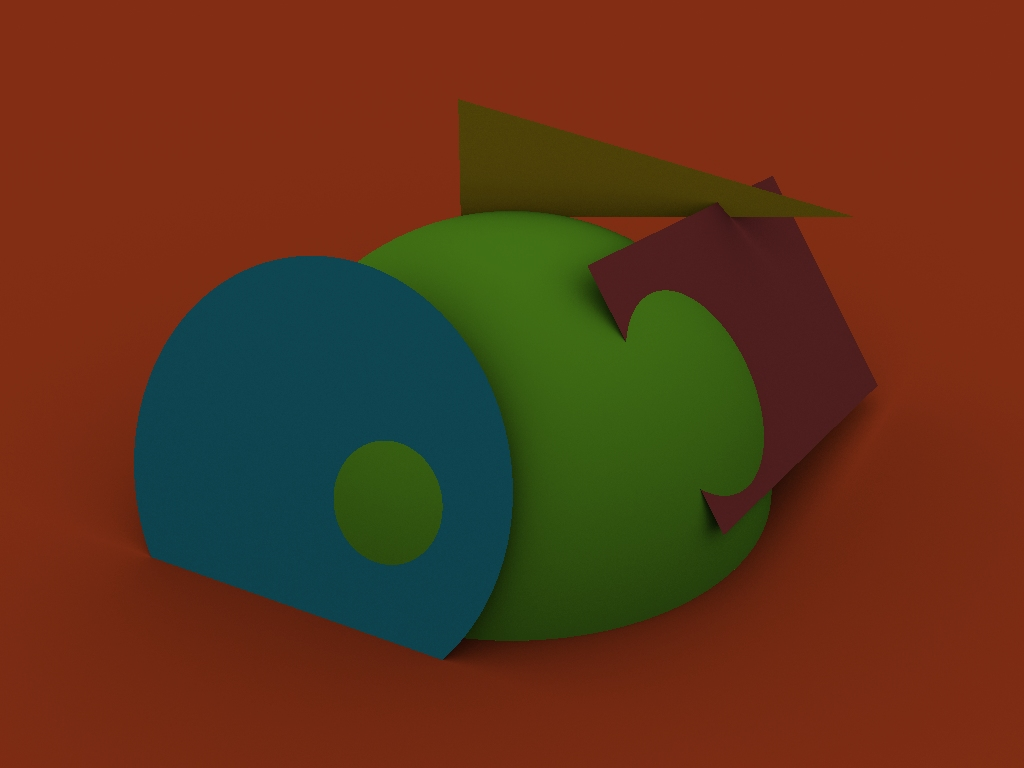
\includegraphics[width=0.8\textwidth]{./img/obj_schnitt/schnitt_objekte.jpg}
    \caption{Schnitt einer Kugel mit Ebene, Scheibe, Rechteck und Dreieck. Der zum Betrachter nächste Schnittpunkt wird zu korrekten Darstellung der Objektdurchdringungen benötigt.}
    \label{fig:schnitt_objekte}
\end{figure}


\section{Ebene}
Der Schnitttest mit einer Ebene gestaltet sich sehr einfach und dient als Grundlage für weitere Schnitttests mit Objekten wie Rechtecken, Dreiecken oder Scheiben. Dazu betrachtet man folgende implizite Form der Ebene:
\begin{equation}
(\boldsymbol{p} - \boldsymbol{a}) \cdot \boldsymbol{n} = 0
\end{equation}
wobei $\boldsymbol{a}$ ein Ortsvektor in der Ebene ist und $\boldsymbol{n}$  eine Normale, die somit senkrecht auf der Ebene steht.
Den impliziten Charakter erhält die Gleichung dadurch, dass sie eine Bedingung an Punkte $\boldsymbol{p}$ in der Ebene stellt. Ein Punkt liegt nämlich genau dann in der Ebene, wenn die Normale $\boldsymbol{n}$ senkrecht auf dem Vektor von $\boldsymbol{a}$ nach $\boldsymbol{p}$ steht und das Skalarprodukt somit gleich Null ist.

Das Ziel ist es jetzt, die Strahlgleichung~\ref{eq:Strahlgleichung} einzusetzen und den Parameter $t$ zu bestimmen, wobei nur für positive \(t\) tatsächlich ein Schnitt vorliegt.


\begin{align}
 0 &= (\boldsymbol{o} + t \cdot \boldsymbol{d} - \boldsymbol{a}) \cdot \boldsymbol{n} 		\nonumber\\
\text{Finale Form:} \qquad t &= \frac{(\boldsymbol{a} - \boldsymbol{o}) \cdot \boldsymbol{n} }{\boldsymbol{d} \cdot \boldsymbol{n} } \label{eq:ebenenschnitt}
\end{align}

Zum Schattieren der Ebene wird die Normale \( \boldsymbol{n} \) verwendet, die bereits zur Definition der Ebene diente. Der Schnittpunkt \( \boldsymbol{r} \) lässt sich nun leicht durch Einsetzen von \( t \) in die Strahlgleichung~\ref{eq:Strahlgleichung} bestimmen, da Strahlursprung \( \boldsymbol{o} \) und Strahlrichtung \( \boldsymbol{d} \) durch das Kameramodell bereits festgelegt sind.


\section{Rechteck}

\FloatBarrier

%\begin{figure}
%    \centering
%    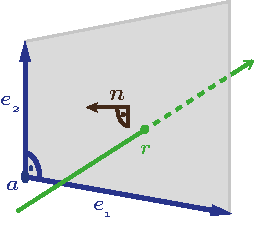
\includegraphics[scale=1.5]{img/obj_schnitt/rechteck.pdf}
%    \caption{Definition Rechteck  }
%    \label{fig:rechteck}
%\end{figure}


\begin{wrapfigure}[18]{r}{0.45\textwidth}    
    \vspace{-15pt}
    \centering
    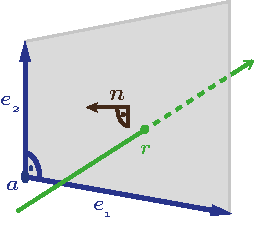
\includegraphics[width=0.44\textwidth]{img/obj_schnitt/rechteck.pdf}
    \vspace{-10pt}
    \caption{Definition eines Rechtecks durch linken unteren Stützpunkt $\boldsymbol{a}$, Kantenvektoren $\boldsymbol{e_1}, \boldsymbol{e_2}$ und Normale $\boldsymbol{n}$. Ein Strahl schneidet das Rechteck am Schnittpunkt $\boldsymbol{r}$.  }
    \label{fig:rechteck}
\end{wrapfigure}


Eine einfache Repräsentation eines Rechtecks besteht darin, den linken unteren Punkt \(\boldsymbol{a}\) anzugeben und die Ausdehnung des Rechtecks durch zwei orthogonal verlaufende Vektoren \(\boldsymbol{e_1}\) und \(\boldsymbol{e_2}\) festzulegen (siehe Abbildung~\ref{fig:rechteck}). Diese Informationen sind bereits ausreichend, um die auf dem Rechteck senkrecht stehende Normale \(\boldsymbol{n}\) durch den Term \( \left( \boldsymbol{e_1} \times \boldsymbol{e_2} \right) \cdot \left( |\boldsymbol{e_1} \times \boldsymbol{e_2}| \right)^{-1} \) zu bestimmen. Dennoch ist es in der Implementation sinnvoll, die explizite Angabe der Normalen zu erlauben, da auf diese Weise festgelegt werden kann, für welche Seite die Schattierungsberechnungen durchgeführt werden soll.


Der eigentliche Schnitttest verläuft nun in zwei Schritten. Zuerst wird ein Ebenen-Schnitttest nach Gleichung~\ref{eq:ebenenschnitt} durchgeführt, wodurch man den Parameter \(t\) erhält. Durch die Strahlgleichung~\ref{eq:Strahlgleichung} lässt sich nun, falls existent, exakt der Schnittpunkt \(\boldsymbol{r}\) berechnen.

Im nächsten Schritt erzeugt man einen Vektor \(\boldsymbol{v}  = \boldsymbol{r} - \boldsymbol{a}\). Diesen projiziert man auf Basisvektoren, die die gleiche Richtung wie \( \boldsymbol{e_1} \) und \( \boldsymbol{e_2} \) besitzen.
Damit erhält man die Länge des Vektors \( \boldsymbol{v} \) in Richtung von \( \boldsymbol{e_1} \) und \( \boldsymbol{e_2} \). Die so projizierten Vektoren \( \boldsymbol{v_{e_1} } \) und \( \boldsymbol{v_{e_2} } \) erhält man daher durch:
\begin{align*}
    \boldsymbol{v_{e_1} } = \frac{ \boldsymbol{v} \cdot \boldsymbol{e_1} }{ |\boldsymbol{e_1}| }  \qquad \qquad \qquad
    \boldsymbol{v_{e_2} } = \frac{ \boldsymbol{v} \cdot \boldsymbol{e_2} }{ |\boldsymbol{e_2}| }
\end{align*}


Der Punkt \( \boldsymbol{r} \) ist genau dann ein Schnittpunkt des Rechtecks, wenn die Längen von \( \boldsymbol{v_{e_1} } \) und \( \boldsymbol{v_{e_2} } \) positiv sind und nicht länger als ihre jeweiligen Projektionsachsen. Daher müssen folgende Ungleichungen gelten:
\begin{align*}
    0 \leq |\boldsymbol{v_{e_1}}| \leq |\boldsymbol{e_1}| \qquad \text{und} \qquad
    0 \leq |\boldsymbol{v_{e_2}}| \leq |\boldsymbol{e_2}|
\end{align*}

Momentan muss noch eine Quadratwurzel berechnet werden, um \( |\boldsymbol{v_{e_1}}| \) zu erhalten. Diese Operation ist jedoch relativ teuer und lässt sich einfach vermeiden, indem man die Ungleichung umformt:
\begin{align}
  \text{Final:} \qquad  0 \leq \boldsymbol{v} \cdot \boldsymbol{e_1}  \leq \boldsymbol{e_1} \qquad \text{und} \qquad
    0 \leq \boldsymbol{v} \cdot \boldsymbol{e_2}  \leq \boldsymbol{e_2}
\end{align}

\FloatBarrier

\section{Scheibe}

Eine Scheibe wird durch drei Komponenten definiert. Dem Mittelpunkt \( \boldsymbol{a} \), einer Normalen \( \boldsymbol{n} \), die senkrecht auf der Scheibe steht und somit deren Lage festlegt, und dem Radius \( r \).
Zuerst wird auch hier ein Ebenen-Schnitttest nach Gleichung \ref{eq:ebenenschnitt} durchgeführt.
Anschließend wird geprüft, ob der Schnittpunkt \( \boldsymbol{r} \) (berechnet durch Gleichung \ref{eq:Strahlgleichung}) in der Scheibe liegt. Der Ebenenschnittpunkt \( \boldsymbol{r} \) liegt in der Scheibe, wenn folgende Ungleichung erfüllt ist:
\begin{equation}
    0 \leq |\boldsymbol{r} - \boldsymbol{a}|^2 \leq r^2
\end{equation}



\section{Dreieck}\label{sec:dreieck}

Der nun folgende Schnitttest wird im Buch "`Physically Based Rendering"' \cite{pharrhumphrey2010Physically} beschrieben und geht zurück auf die Arbeit von Thomas Möller und Ben Trumbore \cite{moller1997FasMinStoRayInt}. Wie bei den bisher vorgestellten Schnitttests könnte man zuerst den Schnittpunkt mit der durch das Dreieck aufgespannten Ebenen berechnen und anschließend durch einen Halbseitentest feststellen, ob dieser Schnittpunkt innerhalb des Dreiecks liegt. Die Methode von \cite{moller1997FasMinStoRayInt} löst dieses Problem allerdings eleganter durch die Verwendung von baryzentrischen Koordinaten, die auf die Arbeit von August Ferdinand Möbius~\cite{mobius1827DerBarCal} zurückgehen. Man erhält dadurch nicht nur die Position des Schnittpunktes im globalen Koordinatensystems, sondern auch dessen Lage innerhalb des Dreiecks, ausgedrückt durch baryzentrische Koordinaten. Letzterer Aspekt wird noch eine wichtige Rolle beim Texturieren von Objekten in Kapitel~\ref{ch:texturierung} spielen. Zudem wird in \cite{moller1997FasMinStoRayInt} gezeigt, dass sich der Speicherverbrauch durch das Vermeiden des Strahl-Ebenen Schnitts verringern lässt.

%\begin{figure}
%    \centering
%    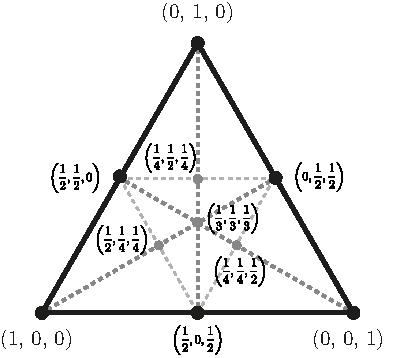
\includegraphics[scale=1]{img/obj_schnitt/baryzentrum.pdf}
%    \caption{Baryzentrische Koordinaten im Dreieck.}
%    \label{fig:baryzentrum}
%\end{figure}


\begin{wrapfigure}[20]{r}{0.45\textwidth}    
    \vspace{-15pt}
    \centering
    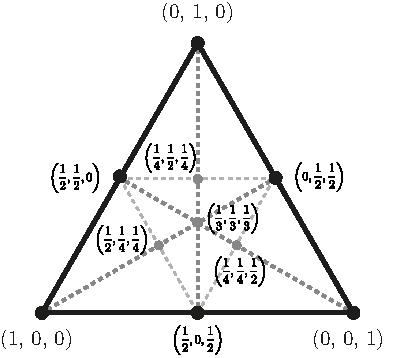
\includegraphics[width=0.44\textwidth]{img/obj_schnitt/baryzentrum.pdf}
    \vspace{-10pt}
    \caption{Baryzentrische Koordinaten im Dreieck. Alle Punkte im Dreieck können als gewichtete Summe der 3 Eckpunkten dargestellt werde.}
    \label{fig:baryzentrum}
\end{wrapfigure} 
 

Ein Dreieck ist gegeben durch drei Punkte \( \boldsymbol{p_0}, \boldsymbol{p_1} \) und \( \boldsymbol{p_2} \). Die Normale \( \boldsymbol{n} \) lässt sich aus dem Kreuzprodukt \( \boldsymbol{n} = (\boldsymbol{p_1} - \boldsymbol{p_0}) \times (\boldsymbol{p_2} - \boldsymbol{p_0})  \) errechnen. Das Ziel ist es nun, einen Schnitt festzustellen und den Schnittpunkt \( \boldsymbol{r} \) durch baryzentrische Koordinaten auszudrücken. Dazu werden die Koeffizienten \( \alpha, \beta \text{ und } \gamma \) eingeführt, die als Gewichte für die Punkte \( \boldsymbol{p_0}, \boldsymbol{p_1} \) und \( \boldsymbol{p_2} \) dienen. Sie besitzen daher die gleiche Bedeutung wie die Massen bei der Bestimmung des Massenschwerpunkts. Der gesuchte Schnittpunkt \( \boldsymbol{r} \) lässt sich somit als gewichtetes Mittel der Dreieckspunkte darstellen:

\begin{equation}
\label{eq:bary}
    \boldsymbol{r} = \alpha \cdot \boldsymbol{p_0} + \beta \cdot \boldsymbol{p_1} + \gamma \cdot \boldsymbol{p_2}
\end{equation}

Da nur Schnittpunkte gesucht sind, die innerhalb des Dreiecks liegen, müssen die Gewichte stets positiv sein. Außerdem gilt für jeden Punkt innerhalb des Dreiecks, dass sich die Gewichte zu \( 1 \) summieren. Es gelten somit die folgenden Bedingungen:

\begin{align}
\label{eq:bary_bedingung1}
\text{Bedingung 1:} &      \qquad 0 \leq \alpha \leq 1;  \qquad 0 \leq \beta \leq 1; \qquad 0 \le \gamma \leq 1 \\
\label{eq:bary_bedingung2}
\text{Bedingung 2:} &      \qquad \alpha + \beta + \gamma = 1 
\end{align}


Die zweite Bedingung \ref{eq:bary_bedingung2} ermöglicht es \( \alpha \) durch \( \beta \) und \( \gamma \) auszudrücken. Nach Einsetzen der Strahlgleichung \ref{eq:Strahlgleichung} für \( \boldsymbol{r} \) ergibt sich folgende Form: 


\begin{equation*}
    \boldsymbol{o} + t \cdot \boldsymbol{d} = (1 - \beta - \gamma) \cdot \boldsymbol{p_0} + \beta \cdot \boldsymbol{p_1} + \gamma \cdot \boldsymbol{p_2}
\end{equation*}

Der nächste Schritt besteht darin, diese Gleichung in eine Form zu bringen, die mit Hilfe der Cramerschen Regel lösbar ist. Sie hat die Form \( \boldsymbol{A} \cdot \boldsymbol{x} = \boldsymbol{b} \), wobei eine Lösung für \( \boldsymbol{x} \) gesucht ist. Nach dem Umformen erhält man:

\begin{equation*}
% Matrix-vector equation with annotated braces
\underbrace{%
    \begin{bmatrix}
        \boldsymbol{d} & \boldsymbol{p_1}-\boldsymbol{p_0} & \boldsymbol{p_2}-\boldsymbol{p_0}
    \end{bmatrix}%
}_{\boldsymbol{A}}
\cdot
\underbrace{%
    \begin{pmatrix} t \\ \beta \\ \gamma \end{pmatrix}%
}_{\boldsymbol{x}}
\;=\;
\underbrace{%
    \boldsymbol{o}-\boldsymbol{p_0}%
}_{\boldsymbol{b}}
\end{equation*}

Abkürzend wird hier nur die resultierende Gleichung zitiert. Die vollständige Herleitung kann in \cite{pharrhumphrey2010Physically} (S. 140 ff) nachgelesen werden.
Mit folgenden Substitutionen

\begin{align*}
    \boldsymbol{e_1} &= \boldsymbol{p_1} - \boldsymbol{p_0};  & \boldsymbol{e_2} &= \boldsymbol{p_2} - \boldsymbol{p_0}; & \boldsymbol{s} = \boldsymbol{o} - \boldsymbol{p_0};\\
    \boldsymbol{s_1} &= \boldsymbol{d} \times \boldsymbol{e_2};   &  \boldsymbol{s_2} &= \boldsymbol{s} \times \boldsymbol{e_1}; &
\end{align*}

sind nun alle Komponenten bekannt, um die finale Gleichung \ref{eq:triangle_final} zu lösen.

\begin{equation}
    \label{eq:triangle_final}
    \text{Finale Form:} \qquad \begin{pmatrix} t \\ \beta \\ \gamma \end{pmatrix} = \frac{1}{\boldsymbol{s_1} \cdot \boldsymbol{e_1} } \cdot
    \begin{pmatrix}
        \boldsymbol{s_2} \cdot \boldsymbol{e_2} \\ \boldsymbol{s_1} \cdot \boldsymbol{s} \\ \boldsymbol{s_2} \cdot \boldsymbol{d}
    \end{pmatrix} 
\end{equation}

Abschließend ist zu bemerken, dass die Berechnung der Gleichung \ref{eq:triangle_final} unter Umständen frühzeitig beendet werden kann, falls kein Schnitt vorliegt. Dazu
verwendet man Bedingung \ref{eq:bary_bedingung1} und \ref{eq:bary_bedingung2} sowie die Tatsache, dass eine Division durch 0 nicht definiert ist.
Algorithmus \ref{alg:dreieck_schnitt} veranschaulicht in welcher Reihenfolge deshalb die einzelnen Komponenten berechnet werden sollten und welche Bedingungen verletzt sein müssen, damit die Berechnungen frühzeitig mit dem Rückgabewert "`false"' beendet werden.

\begin{algorithm}[H]
    \caption{Dreieck Schnitttest}
    \label{alg:dreieck_schnitt}
    \begin{algorithmic}[1]
        \State \(divisor \gets \boldsymbol{s_1} \cdot \boldsymbol{e_1}\)
        \If{\( divisor = 0 \)}
            \State\Return{\textbf{false}}
        \EndIf
        \State \( \beta \gets \boldsymbol{s_1} \cdot \boldsymbol{s} \cdot divisor^{-1} \)
        \If{\( \beta < 0 \; \textbf{or} \; \beta > 1 \)}
            \State\Return{\textbf{false}}
        \EndIf
        \State \( \gamma \gets \boldsymbol{s_2} \cdot \boldsymbol{d} \cdot divisor^{-1} \)
        \If{\( \gamma < 0 \; \textbf{or} \; \beta + \gamma > 1 \)}
            \State\Return{\textbf{false}}
        \EndIf
        \State \( t \gets \boldsymbol{s_2} \cdot \boldsymbol{e_2} \cdot divisor^{-1} \)
        \State\Return{\textbf{true}}   
    \end{algorithmic}
\end{algorithm}


\section{Kugel}

Eine Kugel besitzt einen Mittelpunkt \( \boldsymbol{c} \) und einen Radius \( r \). An alle Punkte \( \boldsymbol{p} \) auf der Kugeloberfläche wird durch die implizite Form folgende Bedingung gestellt:

\begin{equation*}
    (\boldsymbol{p} - \boldsymbol{c}) \cdot (\boldsymbol{p} - \boldsymbol{c}) - r^2 = 0
\end{equation*}

D.h. die Entfernung eines Punktes \( \boldsymbol{p} \) vom Mittelpunkt \( \boldsymbol{c} \) muss genau dem Radius entsprechen. Nach Einsetzen der Strahlgleichung~\ref{eq:Strahlgleichung} in obige Gleichung und Umformen erhält man eine quadratische Gleichung, die z.B. durch die a-b-c-Formel gelöst werden kann:


\begin{align*}
(\boldsymbol{o} + t \boldsymbol{d} - \boldsymbol{c}) \cdot (\boldsymbol{o} + t \boldsymbol{d} - \boldsymbol{c}) - r^2 &= 0 \\
\overbrace{ \boldsymbol{d} \cdot \boldsymbol{d} }^{a} \, t^2
+ \overbrace{ 2 (\boldsymbol{o} - \boldsymbol{c}) \cdot \boldsymbol{d} }^{b} \, t
+ \overbrace{ (\boldsymbol{o} - \boldsymbol{c}) \cdot (\boldsymbol{o} - \boldsymbol{c}) - r^2 }^{c} &= 0
\end{align*}
}

Eine quadratische Gleichung hat typischerweise eine, zwei oder keine Lösung. Dies hängt davon ab, wie der Strahl die Kugel trifft und welche Werte die Diskriminante annimmt. Verfehlt der Strahl die Kugel, gibt es keine Lösung, tangiert er sie, gibt es eine Lösung und wenn er sie durchdringt, gibt es einen Ein- und Austrittspunkt und somit zwei Lösungen. Ein Strahl kann auch innerhalb einer Kugel beginnen, wobei mathematisch zwei Lösungen existieren, jedoch befindet sich der Schnittpunkt einer der Lösungen hinter dem Strahlursprung und ist unbrauchbar. Dies wird deutlich durch den Parameter \( t \), der in diesem Fall einen negativen Wert annimmt. Ähnlich ist der Fall, in dem der Strahl exakt auf der Kugel"=oberfläche beginnt. Es ist somit sinnvoll, einen gefundenen Schnittpunkt nur dann als solchen zuzulassen, wenn \( t > 0 \) gilt. 

Algorithmus~\ref{alg:kugel_schnitt} demonstriert die Vorgehensweise und gibt \textbf{true} zurück bei erfolgreichem Schnitt:

\begin{algorithm}[H]
    \caption{Kugel Schnitttest}
    \label{alg:kugel_schnitt}
    \begin{algorithmic}[1]
        \State \( diskriminante \gets b \cdot b - 4 \cdot a \cdot c  \)
        \If {\(  diskriminante < 0 \)}
        \State\Return{\textbf{false}}
        \EndIf
        \State \( t \gets -b - \sqrt{diskriminante} \cdot (2a)^{-1}  \) \Comment{Teste zuerst die kleinere Wurzel..}
        \If {\( t > 0 \)}
        \State\Return{\textbf{true}}
        \EndIf
        \State \( t \gets -b + \sqrt{diskriminante} \cdot (2a)^{-1}  \) \Comment{.. jetzt die größere Wurzel}
        \If {\( t > 0 \)}
        \State\Return{\textbf{true}}
        \EndIf
        \State\Return{\textbf{false}}     
    \end{algorithmic}
\end{algorithm}

Nun kann man wieder \( t \) in Strahlgleichung~\ref{eq:Strahlgleichung} einsetzen und Schnittpunkt \( \boldsymbol{r} \) berechnen.
Zuletzt fehlt nur noch die Normale am Schnittpunkt. Diese ergibt sich einfach aus:

\begin{equation*}
    \boldsymbol{n} = \frac{\boldsymbol{r} - \boldsymbol{c} } {|\boldsymbol{r} - \boldsymbol{c}|}
\end{equation*}


\section{Selbstschnitt}

Bei den oben beschriebenen mathematischen Herleitungen der Schnitttests bleibt ein Problem verborgen, das erst in der Implementation erkennbar wird. Dabei handelt es sich um den Selbstschnitt. Ein Strahl wird von der Oberfläche eines Objekts ausgesandt und der Schnitttest erkennt fälschlicherweise einen Schnitt mit eben diesem Objekt. Aufgrund von Ungenauigkeiten bei der Berechnung und Darstellung von Fließkommazahlen liefert der Test \( t > 0 \) oft noch falsche Schnitte, weshalb es sich bewährt hat, gegen einen sehr kleinen Wert \( k_\epsilon \) zu testen, also \( t > k_\epsilon \), wobei sich ein Wert von \( 10^{-4} \) für \( k_\epsilon \) bewährt hat.


